\documentclass[12pt]{article}
\usepackage{amssymb,amsmath}

\usepackage[utf8]{inputenc}
\usepackage{graphicx, graphics, epsfig}
\usepackage{epstopdf}
\usepackage{ifpdf}   
\usepackage{amsfonts}
\usepackage{float}
\usepackage[english,russian]{babel}


%\usepackage[pdftex,unicode]{hyperref}
%\usepackage[noend]{algorithm}
%\usepackage[noend]{algpseudocode}
\usepackage{multicol}

\textheight=24cm
\textwidth=16cm
\oddsidemargin=0pt
\topmargin=-1.5cm
\parindent=24pt
\parskip=0pt
\tolerance=2000
\flushbottom
\def\baselinestretch{1.2} 

\title{Определение характеристик пары фермент-субстрат в модели Михаэлиса-Ментен
на основе спектрофотометрических исследований <<чистых>> растворов}
\author{Вишневский~Валерий \texttt{valera.vishnevskiy@yandex.ru}}
\date{20 декабря 2010}

\begin{document}

%\maketitle
\thispagestyle{empty}

\begin{titlepage}
  \begin{center}
  \textsc{\large{Московский Государственный Университет}
  \\[.5cm]
  \normalsize{Факультет Вычислительной Математики и Кибернетики\\
  Кафедра Математических Методов Прогнозирования}}
  \\[4cm]
 
  \large{Отчет по дипломной работе }\\[1.5cm]
 
  {\Large {Параллельная реализация методов поиска скрытых поведенческих
  закономерностей.}} \\[3cm]
  \begin{flushright}
    Вишневский Валерий\\
    группа 517\\
    научный руководитель: Ветров Дмитрий Петрович
  \end{flushright}
  \vfill
  
  Москва, Декабрь 2010
  \end{center}
 \end{titlepage}
 
\newpage
%\tableofcontents
%\newpage


\section{Введение}
В предыдущих работах был программно реализован метод поиска скрытых 
закономерностей в поведенческих данных, основанный на алгоритме, предложенном
М.С.~Магнусоном в~\cite{Magnusson}. Данный метод хорошо зарекомендовал себя, 
однако имел ряд очевидных недостатков. Попытка устранить главный недостаток~--- 
чувствительность к шуму в исходных, была произведена нами введением 
вероятностной модели на паттерн~\cite{MB_article}.

Стоит отметить, что метод Магнусона поиска четких законмернотей 
достаточно вычислительно сложен. Вероятностный подход, эксплуатируемый нами
в методе поиска нечетких паттернов требует еще большего количества вычислений,
что и мотивирует нас на разработку параллельной версии предложенного метода.
\subsection{Поиск четких паттернов}
Дана разметка поведения животного во времени:
\begin{figure}[H]
	\noindent
	\begin{flushleft}
	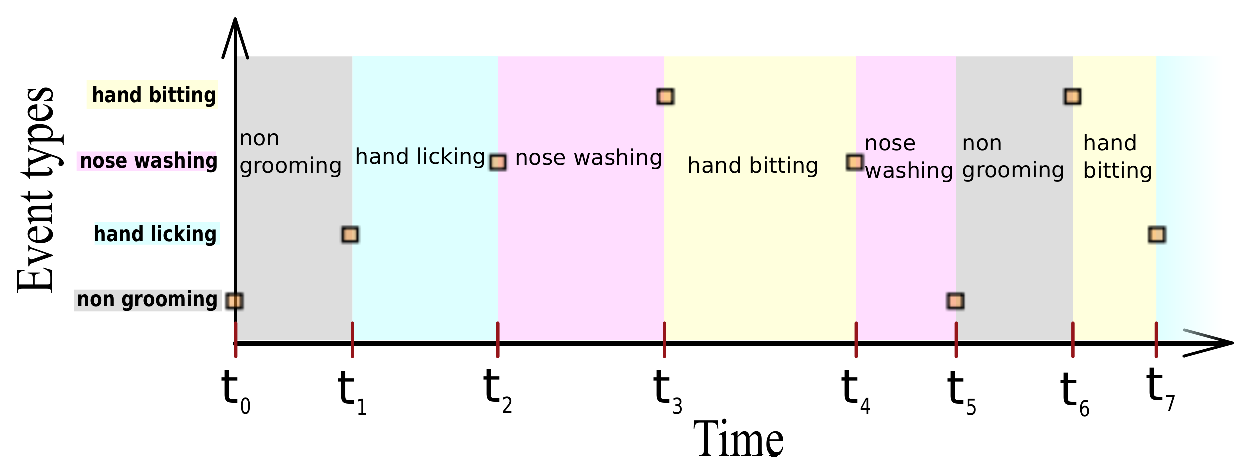
\includegraphics[scale=0.65]{beh_data.eps}
	\end{flushleft}
	\caption{Поведенческие данные.}
\end{figure}

Паттерн~--- это последовательность событий(поведенческих актов), повторяющихся один за другим 
достаточно часто. Для поиска паттернов используется следующая процедура:

Инициализируем множество паттернов псевдопаттернами(поведенческие акты). Потом итеративно повторяем:
  \begin{itemize}
   \item {\bf Конструирование:}Для всех пар паттернов проверить, повторяется ли один за другим достаточно часто. Если да, 
	то получаем новый паттерн.
   \item {\bf Зачистка:} Удалить одинаковые паттерны, которые были сконструированы по-разному.
  \end{itemize}

Ключевым моментом является этап конструирования паттернов. рЗдесь вводится понятие
критического интервала ($A[d_1,d_2]B$)~--- это связь между двумя паттернами, означающая, 
что второй паттерн($B$) промежутке $[d_1,d_2]$ после появления первого паттерна($A$) 
чаще, чем ожидается. Сразу отметим, что в данном определении дискретность вводится
требованием события попасть в интервал $[d_1,d_2]$.

\subsection{Поиск нечетких паттернов}
В этом методе паттерн определяется как последовательность элементарных событий,
где каждое событие паттерна характеризуется смещением и разбросом от предыдущего события(гармошка), 
либо от предыдущего мат. ожидания(занавеска),
$$P=A[\mu_A,\sigma_A]B[\mu_B,\sigma_B]C[\mu_C,\sigma_C]$$
\begin{figure}[H]
	\noindent
	\begin{flushleft}
	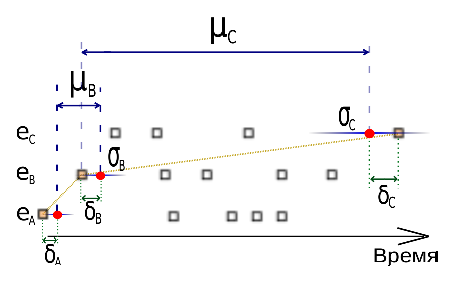
\includegraphics[scale=1.8]{il1.eps}
	\end{flushleft}
	\caption{Представление нечеткого паттерна.}
\end{figure}

Более того, для каждого паттерна длины $N$ мы вводим штраф за пропуск $x$ событий:
  $$
  f_{LOSS}(x,N)= \begin{cases}
   \exp\bigl(-\frac{\lambda x}{N}\bigr), & x < N, \\
   0,                                    & x=N,
   \end{cases}
  $$
 здесь $\lambda$ определяет уровень нечеткости паттернов.
 
Сама процедура конструирования паттернов основанная анализе распределения
межточечных расстояний описана в~\cite{MB_article}.
\section{Ожидаемые результаты}
Будучи, по сути, переборными, оба метода поиска и четких и, тем более, 
нечетких паттернов вычислительно
сложны. Однако в нашем случае основная часть вычислений(подсчет уровней
значимости межсобытийных связей) может быть произведена параллельно, используя
лишь часть исходных данных наблюдений. Именно такие задачи, как показывает
практика(например,~\cite{gpu1, gpu2}), особенно хорошо подходят для реализации
на вычислительной архитектуре GPU(увелечение производительности на порядки: от 10
до 100 раз, в зависимости от задачи и реализации).

Такое увеличение производительности позволит запускать поиск закономерностей 
на более длинных массивах данных, учитывать большее число событий, вести более
глубокий поиск взаимосвязей между событиями.
\section{Проделанная работа}
Для реализации нашего метода на GPU была выбрана платформа CUDA(Fermi) от 
компании NVIDIA. Пока ведется работа по распараллеливанию метода поиска 
четких паттернов. На текущей версии реализован базовый метод определения
критических интервалов в данных. Пока что наблюдается прирост производительности на один
порядок(7-8 раз). Однако стоит заметить, что из-за ограничений платформы 
CUDA по работе с памятью, еще не реализована возможность обработки реальных
длинных поведенческих закономерностей, на которых уже можно более объективно
оценить прирост производительности параллельной версии метода.

\newpage
\begin{thebibliography}{00}
\bibitem{Magnusson}
M.S.~Magnusson. Discovering hidden time patterns in behavior:
T-patterns and their detection.~--- Behavior Research Methods, Instruments, Computers
2000, 32 (I), 93-I IO.

\bibitem{MB_article}
V.V.~Vishnevskiy, D.P~Vetrov. The Algorithm for Detection of Fuzzy Behavioral Patterns
~---Proceedings of Measuring Behavior 2010,ISBN 978-90-74821-86-5 

\bibitem{gpu1}
J.D.~Hall, J.C.~Hart. GPU Acceleration of Iterative Clustering.~---
University of Illinois at Urbana-Champaign, June 4, 2004.

\bibitem{gpu2}
J.~Kruger, R.~Westermann.
Linear Algebra Operators
for GPU Implementation of Numerical Algorithms.~---
Computer Graphics and Visualization Group, Technical University Munich
\end{thebibliography}

\end{document}
